\documentclass[sigchi]{acmart}
\usepackage{algorithm}
\usepackage[noend]{algpseudocode}


\AtBeginDocument{%
  \providecommand\BibTeX{{%
    \normalfont B\kern-0.5em{\scshape i\kern-0.25em b}\kern-0.8em\TeX}}}

\settopmatter{printacmref=false, printccs=false, printfolios =false}
\setcopyright{none} 
\renewcommand\footnotetextcopyrightpermission[1]{}

\acmConference[SDCC Project A.A. 2018-2019]{ }{September 18, 2019}{ }

\begin{document}

\title{Byzantine Fault-Tolerant and Locality-Aware Scheduling MapReduce}

\author{Andrea Graziani}
\email{andrea.graziani93@outlook.it}
\affiliation{%
  \institution{Università Degli Studi di Roma Tor Vergata}
  \city{Rome}
  \state{Italy}
}

\renewcommand{\shortauthors}{Andrea Graziani (0273395)}

\begin{abstract}
\textit{MapReduce} is a programming paradigm developed by Google that enables massive scalability across hundreds or thousands of servers allowing to process very large data-set \cite{IBMWhatIsMapReduce}.

Both academic literature and daily experience shows that \textit{arbitrary faults} frequently occur corrupting our results \cite{BFLMapReduce}. Moreover, ignore data-set locality can lead to performance degradation and a pointless bigger network traffic \cite{LARTS}.

In this paper we present an original MapReduce runtime system capable both to tolerate arbitrary faults and to recognize input data network locations and sizes in order to perform a \textit{locality-aware task scheduling}, improving performance and diminishing network traffic.

Although job's execution using our system requires more resources respect to other implementations, we believe that this cost is acceptable for critical applications that require an higher level of fault tolerance.
\end{abstract}

\keywords{MapReduce, Fault tolerance, Arbitrary failure, Data locality}
\maketitle

\section{Introduction}

Various data-intensive tasks, like seismic simulation, natural language processing, machine learning, astronomical data parsing, web data mining and many other, require a processing power that exceeds the capabilities of individual computers imposing the use of a \textit{distributed computing} \cite{LARTS}.

Nowadays many famous distributed applications use MapReduce framework as solution for processing large data sets in a distributed environment. In order to properly provide services to an increasing number of users worldwide, is necessary to connect together thousands of computers and hundreds of other devices like network switches, routers and power units, moving consequently an huge amount of data between computers. 

However, as many studies confirm, \textit{hardware component failures are frequent} and they will probably happen more often in the future due to increasing number of computers connected to internet \citep{BFLMapReduce}. Is been documented that in the first year of a cluster at Google there were 1000 individual machine failures and thousands of hard drive failures \cite{PetaScaleFailure}. A recent study of DRAM errors in a large number of servers in Google data-centres for 2.5 years concluded that these errors are more prevalent than previously believed, with more than 8\% DIMM affected by errors yearly, even if protected by error correcting codes (ECC) \cite{DRAMError}. A Microsoft study of 1 million consumer PCs shown that CPU and core chipset faults are also frequent. \cite{MicrosoftStudyFailure} Moreover moving large amount of data repeatedly to distant nodes is becoming the bottleneck owing to an increased network traffic causing performance degradation.

Therefore to construct a distributed system capable to provide its services even in the presence of failures is become so critical; consequently, to provide a \textit{fault tolerant} cloud application represents an important goal in distributed-systems design. 

Moreover, due to very large data-set involved during data-intensive tasks, exploiting data locality, in order to mitigate network traffic and delay, becomes very important to improve performance.

In these paper we will describe our \textit{Arbitrary Fault-Tolerant Locality-Aware} (AFTLA) MapReduce system capable to resolve all issues described above. We have implemented an AFTLA MapReduce system, capable to perform a word-count of a given text input, from scratch using Go programming language, adopting Apache ZooKeeper\textsuperscript{TM} for maintaining configuration information and system coordination \footnote{See \url{https://zookeeper.apache.org}}; all libraries used in our implementation are fully described in table \ref{tab:libraries}. Our prototype    's source code is fully available on GitHub\footnote{See \url{https://github.com/AndreaG93/SDCC-Project}}, famous web-based hosting service for version control using \texttt{git}; we remind that \LaTeX\ source code of this paper is available too\footnote{See \url{https://github.com/AndreaG93/SDCC-Project-Report}}.  


\begin{table*}
  \caption{Libraries used in our implementation}
  \label{tab:libraries}
  \begin{tabular}{l|l|l}
    \toprule
    Name & Description & Link \\
    \midrule
    \texttt{go-zookeeper/go} & Native Go Zookeeper Client Library & \url{https://github.com/samuel/go-zookeeper} \\
    \texttt{logrus} & A structured logger for Go & \url{https://github.com/Sirupsen/logrus} \\
    \texttt{aws-sdk-go} & AWS SDK for the Go programming language. & \url{https://github.com/aws/aws-sdk-go} \\
    \bottomrule
  \end{tabular}
\end{table*}

\section{Assumptions}

In order to properly describe how our algorithm can tolerate arbitrary faults and to exploit data locality, it is necessary to describe its architecture. To do that, in this section we start making some very important assumptions.

Our system is composed by a \textit{set of distributed processes}, every of which run on different hosts in a same data-center; in our prototype, every process run on his own Amazon EC2 server hosted in a same region (\texttt{us-east-1}). All processes interact with each other using RPC

We assume that our system runs \textit{asynchronously}, that is no assumptions about process execution speeds or message delivery times are made; therefore we can normally use timeouts to state that a process has crashed although, occasionally, such conclusion is false \cite{SDCC}.

All processes are connected by \textit{reliable channels}, so no messages are lost, duplicated or corrupted; that feature is guaranteed by TCP connections. All system processes use RPC protocol in order to interact with each other.

Clients are \textit{always correct}, because if they are not there is no point in worrying about the correctness of our system's output. Finally we assume the existence of an hash function that is \textit{collisions-resistant}, for which it is infeasible to find two inputs that produce the same output.

In this paper, we take for granted reader's knowledge of the MapReduce framework and Hadoop implementation. framework.

\section{System's model}

\begin{figure}[h]
  \centering
  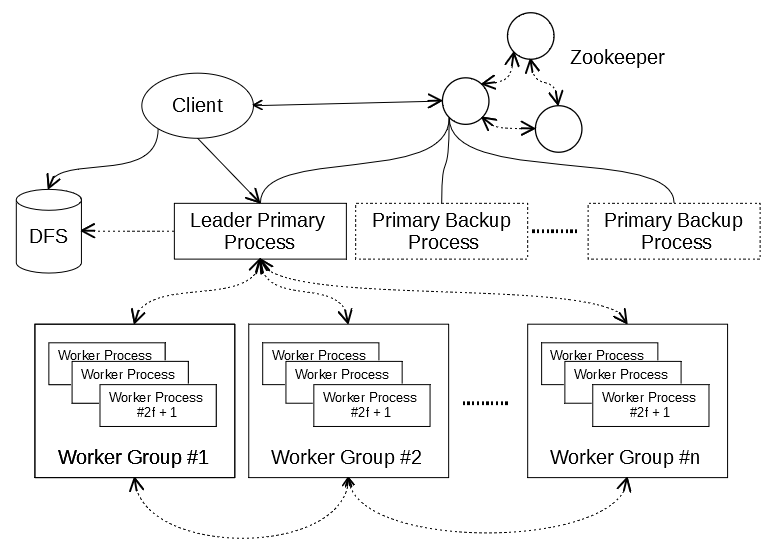
\includegraphics[width=\linewidth]{Architecture}
  \caption{System Architecture}
\end{figure}

Three kind of process are used in our system:

\begin{description}
\item[Client Processes] Which send word-count requests to our system sending directly an input text file. 

\item[Worker Process (WP)] They execute \textit{map} or \textit{reduce} scheduled by LPP.

\item[Primary Process (PP)] It is similar to \textit{JobTracker} process used in Apache Hadoop which duty is to satisfy clients requests scheduling \textit{map} or \textit{reduce} tasks. 
\end{description}

\subsection{Primary Process}
At this point, is necessary to make some clarifications about PP's features.

Unlike Hadoop, according to which \textit{JobTracker} process is assumed always correct, the host where PP is running may fail, for example by crashing or by losing network connectivity; in other words, as known in academic literature, PP represents a \textit{single point of failure}.

Therefore, to ensure an high system availability, adopting the same design used in Apache Mesos\textsuperscript{TM}\ \footnote{See \url{http://mesos.apache.org/documentation/latest/architecture/}}, our system architecture is based on multiple PP backup copies run on different machines; using any leader election algorithm, is possible to elect one of these copies as \textit{Leader Primary Process} (LPP) while all the others remain on stand-by. Using this approach, is possible to manage PP crash failure: when current leader fails, a backup copy is promoted to become the new . 

LPP represents our system coordinator since only it can can interact with WP scheduling task using a \textit{push-based} approach (unlike Hadoop according to which JobTracker schedules task using a \textit{pull-based} approach \cite{LARTS})

However, to perform its task, LPP manages various information about clients requests, many of which, as we will see later, are sent by WP after a map or reduce task. In other word, LPP has got a status.

Is very important to specify that LPP status is stored in memory, therefore they are permanently lost after a crash; this design makes our system easier to implement and helps to reducing overhead due to the disk I/O activities. However recover lost in-memory leader state after a failure is required in order to satisfy clients requests. 

Therefore we have adopt a design according to which LPP make a sort of backup, or snapshot, of its current state regularly. To make our implementation easier, in our prototype, considering that LPP state contains a very small amount of data, LPP stores its state in a Zookeeper cluster after some events, like a map task termination. In case of crash failure of current LPP, when a primary process backup becomes leader, it retrieves all data from Apache ZooKeeper cluster, recovering last saved state.

\subsection{Worker Process and Groups}

To make WP arbitrary fault-tolerant we have adopt a design according to which each task (map, reduce, etc.) is executed more than once by different processes running on different host. This approach requires to organize all our WPs into several \textit{groups} through which became possible to mask one or more faulty processes of a given group. 

Before explaining how we manage WP faults, we must explain what is a Worker Processes Group (WPG). A WPG is a set of identical worker processes, each of which execute, relatively to a given job, \textit{the same commands using the same input data in the same order}; therefore we expected that all WPs belonging to a same group would produce the same output when no arbitrary fault occurs. All commands and data are sent by LPP.

Suppose to want tolerate at most $f$ arbitrary failures of all WPs belonging to a given group. 

To achieve that level of fault-tolerance, we can apply to reach, for instance, \textit{byzantine agreement} among all processes belonging to group. However we believe that solution is too expensive because it requires, as properly explain in literature\citep{SDCC}, $3f + 1$ replicas.

Therefore we have adopt a protocol based on \textit{majority voting} inspired to quorum-based protocols applied in replicated-write systems. As explained in literature\citep{SDCC}, in this kind of systems, if processes exhibit arbitrary failures, continuing to run when faulty and sending out erroneous or random replies, a minimum of $2f+1$ processes are needed to achieve $f$-fault tolerance. In the worst case, the $f$ failing processes could accidentally generate the same reply. However, the remaining $f+1$ will also produce the same answer, so the LPP just believes the majority.

In our design each map or reduce task scheduled by current LPP are assigned to independent WPGs. Let's try to explain this statement formally using map task as example (but is the same of any task). Let $i = 1,2,3...n$, where $n \in \mathbb{Z}_+$. As MapReduce framework states, our system splits the input text file $S$ in $n$ parts $\lbrace s_1, s_2, ... s_n \rbrace$ called \textit{split}; each split $s_i$ is associated to a map task $m_i \in \lbrace m_1, m_2, ... m_n \rbrace$ every of which must be replicated on multiple WPs to make them arbitrary fault tolerant. Each map task $m_i$ is assigned to a different WPG $g_i \in \lbrace g_1, g_2, ... g_n \rbrace$. As we will explain later, LPP, checking received outputs from each group, we can achieve arbitrary fault tolerance for every scheduled task. Obliviously to tolerate at most $f$ arbitrary failures of each task, each WPG must contains at least $2f+1$ different processes. Then our design requires at least $n(2f+1)$ different WPs.

This design is scalable in several ways: if the number of users or data input size grows, it should be possible to extend the system, at reasonable cost, adding more WPGs. If we want an higher level of arbitrary fault-tolerance, we should add more WP to each WPG, increasing the number PP backups too.

\section{The algorithm}

Given the system model described previously, a solution to tolerate at most $f$ arbitrary faults during each task would be the following: current LPP assigns a given map/reduce task to a WPG contacting its $2f + 1$ WPs; then, after retrieving the outputs from replicas, picks the most voted results which is expected correct if no more than $f$ arbitrary faults occur. 

This simplistic solution is very expensive because it replicates everything $2f + 1$ times: task execution, communication of map task outputs and so on. We use a set of techniques to avoid these costs and do things efficiently:

\subsection{Digest outputs} As explained above, in order to consider a map/reduce task correct, tolerating at most $f$ faulty processes, $f + 1$ matching outputs, coming from at least $2f + 1$ WPs belonging to a given WPG,  have to be received. 

To validate task's output, since outputs computed by worker processes can be very large, in order to avoid pointless additional network traffic, we have adopted an approach according to which LPP fetches and compares \textit{digests}, a bit string of a fixed size obtained using a hash function. The main advantage of this technique is that, digest size are many times smaller than task's data output, allowing us to reduce network traffic among servers, increasing system's performance.

\subsection{Deferred execution} We believe that there is no point in always executing $2f + 1$ replicas for each task to usually obtain the same result. 

To minimize both the number of copies of tasks executed and the overhead due to network traffic we have adopted a design called \textit{deferred execution}: according to that solution current LPP starts only $f + 1$ replicas of the same task, checking if they all return the same result. If a time-out elapses, or some returned results do not match, more replicas (up to $f$) are started, until there are $f + 1$ matching replies. 

We believe that this this design is also energy-saver and cost-effective since, supposing that arbitrary faults are uncommon, fewer WP are involved into computations respect to basic scheme and, in principle, is possible to start and use a fewer number of servers using auto-scaling techniques (at cost of some latency).

\subsection{Data locality awareness}

Since in order to achieve fault tolerance we have replicate all task $2f + 1$ times, data transfers among servers are replicated too, generating an huge amount of network traffic. Evidently, when large data set are involved, move data repeatedly among server became a bottleneck.

Therefore we have adopted a design aware of data locations and sizes capable to reduce the overall amount of transferred data; that solution is based on a basic principles which states that "\textit{moving computation towards data is cheaper than moving data towards computation}"; in other words  "\textit{moving computation towards data is cheaper than moving data towards computation}".

To be more precise, when a WP complete a map task, it send as output to LPP two very important information: a string containing data output digest and a value representing output data size. According to Hadoop terminology, map task output are called \textit{partition} and, contrary to splits, they are of variable sizes: so why not just shuffle smaller partitions instead big one? 

Assume for simplicity that no faults occurs and to have only two WPGs $\lbrace g_1, g_2 \rbrace$. Let $P_{i:g_i}$ the partition owned by WPG $g_i$ which contains all key-value pairs which must be submitted to reduce task $R_i$. The problem is how to perform a locality-aware reduce task scheduling; in other word, which WPG $g_i$ have to run reduce task $R_i$ reducing shuffled data?

Suppose that $P_{1:g_1}$, $P_{2:g_1}$, $P_{1:g_2}$ and $P_{2:g_2}$ have a size of 300 MB, 150 MB, 150 MB and 300 MB respectively. Clearly, scheduling $R_1$ at $g_1$ and $R_2$ at $g_2$ reduce the amount of transferred data among WPGs by 50\%. Obliviously using this approach is possible to perform a locality-aware shuffle task capable to reduce network traffic, applying locality to reduce task scheduling.  

\section{Implementation}

In this last section we will describe some main aspect of our implementation.

\subsection{Crash failure detection} To guarantee the correct functioning of the system, is critical to be able to detect WP and PP crash failure. To resolve this problem we have exploited some features of Apache Zookeeper. 

As known, Apache ZooKeeper has the notion of \textit{ephemeral nodes}, special znodes which exists as long as the \textit{session} that created the znode is active. When session expiration occurs, Zookeeper cluster will delete all ephemeral nodes owned by that session and immediately notify all connected clients of the change.

When any client establishes a session with a Zookeeper cluster, a time-out value is used by the cluster to determine when the client's session expires. Expirations usually happens when the cluster does not hear from the client within the specified session time-out period (i.e. no heartbeat).

Therefore using that feature, we adopted a very simple design according to which any process must to "sign up" creating his own ephemeral node in Zookeeper Cluster in known paths (note that znode paths of PPs and WPs are different in order to not interfere with leader election of PPs). 

It will be the responsibility of LPP to watch for WP's ephemeral node deletions; this approach makes WP status checking very simple. System coordination and membership is facilitated too, since any ephemeral node is used to store information about process that created (ID, Group ID etc.).

\subsection{Primary process leader election algorithm}

\begin{algorithm}
\caption{}\label{alg:leaderElection}
\begin{enumerate}

\item Let \texttt{ROOT} be a valid znode path. Any PP, which wants to become leader, creates a new znode $Z$ with path \texttt{ROOT/$x$}, where $x$ is a number. Using both \texttt{SEQUENCE} and \texttt{EPHEMERAL} flags, $x$ will be the sequence number greater than any one previously used.

\item Let $C$ be the children of \texttt{ROOT}. 

\item If $Z$ is the smallest node in $C$, that is $x$ is the smallest sequence number used so far, then the PP that created $Z$ will become leader.

\begin{enumerate}

\item Otherwise watch for changes on znode \texttt{ROOT/$j$} in C, where $j$ is the largest sequence number such that $j$ < $x$.

\item Upon receiving a notification of znode deletion, go to step number 2. 

\end{enumerate}
\end{enumerate}
\end{algorithm}

Let's now describe in details how we have resolved leader election problem of a PP using Apache Zookeeper.

Suppose that \texttt{ROOT} is a valid path of an existing znode. To apply as possible leader, any PP creates a znode child into \texttt{ROOT} using \texttt{SEQUENCE} and \texttt{EPHEMERAL} flags. When \texttt{SEQUENCE} is used, ZooKeeper cluster automatically appends a sequence number to the new znode that is greater than any one previously appended to a child of \texttt{ROOT}. The PP, which created the znode with the smallest appended sequence number, become leader.

Obliviously is important to watch for failures of the leader in a such way that a new PP arises as the new leader when leader fails. Note that, since we have used \texttt{EPHEMERAL} flag during znode creation, when leader fails the smallest znode will be deleted by Zookeeper cluster. if we make sure that all PPs watch for the next znode down on the sequence of znodes, if a PP receives a notification that the znode it is watching is gone, then it becomes the new leader since there is no smaller znode. 

A complete description of leader election algorithm is shown in Algorithm \ref{alg:leaderElection} while our implementation is in \texttt{SDCC-Project/aftmapreduce/cloud/zookeeper}












\bibliographystyle{ACM-Reference-Format}
\bibliography{Bibliography}

\appendix

\end{document}
\endinput

